%% LyX 2.0.2 created this file.  For more info, see http://www.lyx.org/.
%% Do not edit unless you really know what you are doing.
\documentclass[11pt,twoside]{report}
\usepackage[utf8]{inputenc}
\usepackage{listings}
\usepackage{geometry}
\geometry{verbose}
\setcounter{secnumdepth}{3}
\setcounter{tocdepth}{3}
\usepackage{color}
\usepackage{graphicx}
\usepackage[unicode=true,pdfusetitle,
 bookmarks=true,bookmarksnumbered=false,bookmarksopen=false,
 breaklinks=false,pdfborder={0 0 1},backref=section,colorlinks=true]
 {hyperref}
\hypersetup{
 linkcolor=black,filecolor=black,citecolor=black,urlcolor=black}

\makeatletter
%%%%%%%%%%%%%%%%%%%%%%%%%%%%%% User specified LaTeX commands.
\@ifundefined{definecolor}
 {\usepackage{color}}{}
% ----------------------------------------------
% IT2901 - Informatikk Prosjektarbeid II
% Norwegian University of Science and Technology
% ----------------------------------------------


%\setlength{\oddsidemargin}{5mm}
%\setlength{\evensidemargin}{25mm}
%[top=4.cm, bottom=4.5cm, left=3.cm, right=3.cm]
\usepackage{lumalayout}% Custom fancy layout fra hælvette
% Unicode for norske tegn
% Støtte for bilder inkl. pdf
\usepackage{nameref}% Støtte for labels på kapittel og seksjoner
\usepackage[table]{xcolor}\usepackage{colortbl}% Kolonne farge i tabeller
\usepackage{multirow}\usepackage{parskip}\usepackage{tabularx}\usepackage{umoline}\usepackage{pifont}\usepackage{listings}\usepackage{float}\usepackage{caption}\usepackage{appendix}\usepackage{fixltx2e}\@ifundefined{definecolor}{\usepackage{color}}{}


% Lenker !! Må være til slutt !!
\usepackage[xindy]{glossaries}

% Custom commands ------------------------------------------------------------ %
% Her kan vi legge inn kommandoer for ord og uttrykk, som forekommer ofte i
% rapporten. På den måten får vi uttrykt oss mer konsistent gjennom rapporten, 
% pluss at det blir enklere for oss å forandre på formatteringen av viktige ord
% underveis (f.eks at vi plutselig bestemmer oss for at ntnu skal skrives i
% kursiv eller med fet skrift).
%
% Vi kan prøve å følge en konvensjon her også. Et forslag:
%
%     Kommandoer med små bokstaver -> Full beskrivelse av ordet/uttrykket
%     Kommandoer med store bokstaver -> Forkortelser
%
% Eksempel: 
%
%    \ntnu -> Norwegian University of Science and Technology
%    \NTNU -> NTNU

\newcommand{\project}{oSNAP}

\newcommand{\HRule}{\rule{\linewidth}{0.5mm}}

\newcommand{\todo}[1]{\textbf{[TODO: {\color{red}#1}]}}

%\newcommand{\redcell}[1]{\cellcolor{red!80!yellow}#1}
%\newcommand{\grncell}[1]{\cellcolor{green!40!yellow}#1}
%\newcommand{\ylwcell}[1]{\cellcolor{yellow}#1}

% Custom settings ------------------------------------------------------------ %
% listings defitions
\definecolor{javared}{rgb}{0.6,0,0} % for strings
\definecolor{javagreen}{rgb}{0.25,0.5,0.35} % comments
\definecolor{javapurple}{rgb}{0.5,0,0.35} % keywords
\definecolor{javadocblue}{rgb}{0.25,0.35,0.75} % javadoc

\newcommand{\javacode}{\lstset{language=Java,
basicstyle=\scriptsize\ttfamily,
keywordstyle=\color{javapurple}\bfseries,
stringstyle=\color{javared},
commentstyle=\color{javagreen},
morecomment=[s][\color{javadocblue}]{/**}{*/},
numbers=left,
numberstyle=\tiny\color{black},
stepnumber=1,
numbersep=4pt,
tabsize=4,
showspaces=false,
showstringspaces=false,
breaklines=true}}

\newcommand{\ccode}{\lstset{language=C++,
basicstyle=\scriptsize\ttfamily,
keywordstyle=\color{Blue},
stringstyle=\color{BurntOrange},
commentstyle=\color{Gray},
numbers=left,
numberstyle=\tiny\color{black},
stepnumber=1,
numbersep=10pt,
tabsize=4,
showspaces=false,
showstringspaces=false,
breaklines=true}}





\DeclareGraphicsExtensions{.pdf, .png, .jpg, .gif}
\graphicspath{{./img/}}

\setlength{\headheight}{15pt}



\input{./files/glossary}
\makeglossaries








\makeatother

\begin{document}
% ---------------------------------------------------------------------------- %
% Title page, table of contents, list of tables and figures goes here


\begin{titlepage}
	\begin{center}
		\includegraphics[width=0.5\textwidth]{img/NTNTU-logo.png}\\[1cm]    
		\textsc{\Large IT2901 - Informatics Project II}\\[0.5cm]
		\HRule \\[0.6cm]
		{ \huge \bfseries \project}\\[0.4cm]
		open Social Network Arduino Platform
		\HRule \\[1.5cm]
		\begin{center} \large
			Emanuele \textsc{Di Santo} \\
			Anders \textsc{Behne Eie} \\
			Henrik \textsc{Goldsack} \\
			Johan \textsc{Jansen} \\
			Asbjørn \textsc{Lucassen} \\
			Jonas \textsc{Svarvaa} \\
			Bjørnar \textsc{Håkenstad Wold}
		\end{center}
		\vfill
		{\large \today}
	\end{center}
\end{titlepage}


\cleardoublepage{}\tableofcontents{}\cleardoublepage{}

\listoffigures
\cleardoublepage{}

\listoftables


%\printglossaries
%\newpage


% ---------------------------------------------------------------------------- %
% Main report body goes here
\cleardoublepage{}


\chapter{Introduction}

\label{ch:introduction} \section{Problem description}

\emph{This is the problem description, as per the customer's request.}

Social networking sites such as Facebook\cite{link:facebook} and Twitter\cite{link:twitter}
have normally been accessed  via a web browser. Lately mobile versions have become popular,
and allow access to context data such as location of users. We foresee a much greater popularity
of mobile and pervasive interfaces to social media in the coming years.

Arduino\cite{link:arduino} is a platform that allows software to be written in order to construct
hardware prototypes. In this task the students will develop an Arduino-based interface to Facebook.
The information from Facebook will be made available on Arduino displays and the user can interact
with Facebook through Arduino sensors and actuators.

In case Facebook data access shows to be difficult, the students will use Shindig\cite{link:shinding} which 
is an open source implementation of OpenSocial\cite{link:opensocial} APIs. The service specification is developed
in the European project SOCIETIES in collaboration with European partners. The students are however expected to
innovate and come up with new concepts, user interfaces, and service organization.

\section{The context}
In the past few years, social networks have become more and more popular, continuously increasing their user-base.
The project task was to design and develop an open source Android\cite{link:android} framework for allowing quick
and flexible development of wireless Tangible User Interfaces (TUI) for social networks using Arduino.
The product has served both as a proof-of-concept and as a starting point for future software projects.

\section{The customer}
Our customer was SINTEF, represented by Mr. Babak A. Farshchian.

SINTEF is the largest independent research organization in Scandinavia\cite{link:sintef}.
It is an independent, non-commercial organization with their head office in Trondheim.
They have approximately 2100 employees, mainly in Trondheim and Oslo.

\section{The team}
The team consisted of six students from NTNU and one exchange student.
About half of the members have worked together on previous projects and thus shared
some teamwork skills and experiences. None of the team members had worked for a customer before.

\subsection{Team members}

\begin{itemize}
\item{\anders}\newline
Third year Informatics student at NTNU. Experience with the programming languages Java,
C and C++. Also experience with Arduinos, AVRs and some basic electronics knowledge.

\item{\henrik}\newline
Third year student at NTNU. Main language Java, basic knowledge in 3D and electronic circuits.

\item{\johan}\newline
Third year student at NTNU. Experience with the programming languages Java, C, C++  and
Basic. Worked with AVR micro-controllers in other projects and courses.

\item{\asbjorn}\newline
Second year student on bachelor in computer science at NTNU. Has previously had one year of
introductory psychology which is to be included in the bachelor in computer science.
Experience with Java.

\item{\emanuele}\newline
Third year Computer Science exchange student from Tor Vergata University, Rome.
Experience with Java, C and C++ programming, basic electronic notions.

\item{\jonas}\newline
Third year student at NTNU. Experience with Java, Python, Lua, PHP, and web standards such as HTML, 
CSS and Javascript. Previously worked with media production and sound engineering.

\item{\bjornar}\newline
Third year Informatics student at NTNU. Experience with programming in Java, C and C++.
Previously worked with electronics and have basic knowledge about AVR micro-controllers through
own projects.
\end{itemize}

\section{Definitions}

Here we introduce a list of the terms used in this document with a short explanation of their meaning.

\begin{description}

\item[Android:]
	An operating system based on Linux primarily for mobile devices. It features a software stack, and applications are written in the Java language. Android is made by Google and the Open Handset Alliance.
\item[Android-Arduino applications:]
	With this term we refer to Android applications used to control the behavior of Arduino-based tangible user interfaces.
\item[Apache:]
	A software foundation focused on open source and community driven software.
\item[Arduino:]
	Arduino is a tool for making computers that can sense and control more of the physical world than your
	desktop computer. It's an open-source physical computing platform based on a simple micro-controller board, and a development
	environment for writing software for the board. 
\item[Facebook:]
	Facebook is the biggest social network. It is also the network our libraries primarily focus on.
\item[IPC:]
	Remote Method Invocation in Java (RMI) or Remote Procedure Call in C (RPC) are two implementations of inter-process communication (IPC).
	This allows two different computer programs (possibly on two entierly different systems or platforms) to execute code in their respective
	address space.
\item[JSON:]
	Acronym for Javascript object notation. It is a lightweight data interchange format,
	used in most social networks.
\item[MVC:]
	Acronym for the Model, View, Controller pattern. It's a design pattern used to abstract the data model, logic and presentation.
\item[OpenSocial:]
	OpenSocial is an open source standard by Google for a set of API. It's aim is to
	provide a common runtime environment for web applications within different social networks. It is supported by networks
	such as Orkut, MySpace, LinkedIn and many more, except Facebook and Twitter.
\item[oSNAP:]
	The code name for this project. Acronym for Open Social Network Arduino Platform.
\item[Product:]
	This project's deliverables: a set of prototypes and Android applications and libraries.
\item[Prototype:]
	An Arduino board, running a custom firmware, acting as a tangible user interface.
\item[REST:]
	A software architecture for distributed systems. Software that complies with REST constrains is called RESTful.
\item[RPC:]
	See IPC.
\item[RMI:]
	See IPC.
\item[Shield:]
	An Arduino chip (or module) one puts on top of the main board to extends the arduino's feature set.
\item[Shindig:]
	Shindig is Apache's implementation of the OpenSocial standard.
\item[Social service/applications:]
	With this term we refer to Android applications, used to fetch data from a social network.
\item[TUI:]
	Acronym for tangible user interfaces.
\item[Twitter:]
	World's biggest micro-blogging network.
	
\end{description}


\cleardoublepage{}


\chapter{Team Management}

\label{ch:team} \section{Communication}


Skype, meetings, etc etc





\section{Time management}

schedules, weekly meeting times etc etc etc

\cleardoublepage{}


\chapter{Requirements}

\label{ch:requirements} 
\section{Preliminary requirements}
\begin{itemize}
\item Wireless connectivity 
\end{itemize}
Since the product will target a user-base with no technical background,
the customer required all connections between devices to be wireless,
so that connecting the User Interface to the Android mobile will be
as easy as possible for the end-users. For this reason, the technical
details of the connection should be hidden to the end-user so that
the product can be easily operated. 
\begin{itemize}
\item Flexible software architecture 
\end{itemize}
The software that will be developed for this project will serve as
a proof-of-concept and possibily as a starting point for other research
projects. For this reason a flexible, modular software architecture
is an important requirement for our customer. The code shall be developed
in independent, thus reusable modules so that adding new functionality
will be fairly easy for new developers. 
\begin{itemize}
\item Software licenses 
\end{itemize}
The customer made clear that the software developed needs to be released
under a permissive, Apache compatible software license. This implies
that pre-existing software that will eventually be adopted and incorporated
in the project must have a compatible license. 
\begin{itemize}
\item Working prototype 
\end{itemize}
To show that the concept of Tangible User Interfaces for Android applications
(including social networks) using Arduino is not only possible, but
also a feasible market product, the customer is interested in a working
prototype. As the project evolves, together with our customer we will
gradually decide on the specifications of the prototype that will
be produced at the end of the project. Such prototype will play an
important role for the customer satisfaction. 


\cleardoublepage{}


\chapter{Process Management}

\label{ch:management} \section{The choice of development process}
The choice of a development process is crucial for every project~\cite{book:software-engineering} 
and many factors such as project size and scope, team members skills and time resources have to 
be taken into consideration in order to make a good choice. The choice of the development process 
will affect planning and many other aspects of the teamwork. The following section describes
which development processes we have considered using and the reasons behind our final choice.

\subsection{Waterfall}
The Waterfall model (figure \ref{fig:designmodel-waterfall}) is a strict top-down design process. It features detailed planning, design and
documentation before design. This model is useful when going back and changing requirements is
costly or impossible. This does however require that all needed features and requirements are known
early on. The model was originally used for hardware design and when the first software projects 
appeared it was simply adapted. Many argue that the Waterfall model is bad for software design, seeing
as the developers cannot predict all problems or additional requirements before reviewing a working
prototype of the final product. Customers also often have changing requirements under development.
The Waterfall model works best for expensive projects where problem prediction and initial correct design
is vital before implementation is started.
\begin{figure}[h!]
\centering \includegraphics[scale=0.30]{img/designmodel-waterwall} \caption{The Waterfall model~\cite{link:wiki}}
\label{fig:designmodel-waterfall}
\end{figure}

\subsection{Scrum}
Scrum is an Agile software development process. The Scrum approach uses repetitive iterations (called
Sprints in the Scrum etymology) to design, implement and refine a product. Figure \ref{fig:designmodel-scrum} shows
how the Scrum iterative process works. Each iteration improves, fixes and adds new features to the previous iteration.
A key feature of Scrum is that the customer can change their mind on what they want or need. Scrum focuses on frequent 
group meetings and splitting big tasks into smaller, manageble tasks for small groups of programmers. Because of the
frequent meetings it promotes verbal communication in the group.
\begin{figure}[h!]
\centering \includegraphics[scale=0.4]{img/designmodel-scrum} \caption{The Scrum process~\cite{link:wiki}}
\label{fig:designmodel-scrum}
\end{figure}

\subsection{Extreme Programming (XP)}
Extreme Programming (figure \ref{fig:designmodel-xp}) is a development methodology that is designed for best software quality and
quick responsivness to changing customer requirements. It is also an Agile Development method like
Scrum and therefore shares certain similarities to that development method. It promotes rapid
development and allows the customer to change his/her mind or request new features throughout
the development of the software. Typical elements for XP are pair programming, unit testing,
lazy programming, simplicity and expecting changes in customer requirements as time passes
and the problem is better understood. Several pitfalls include buggy and unstable code or lack of
overall design specification. Extreme programming is best suited for small projects for prototyping
where the customer is not entierly sure what he or she wants.
\begin{figure}[h!]
\centering \includegraphics[scale=0.75]{img/designmodel-xp} \caption{Extreme Programming~\cite{link:xp}}
\label{fig:designmodel-xp}
\end{figure}

\subsection{Agile Unified Process}
The AUP (short for Agile Unified Process) shown in figure \ref{fig:designmodel-aup} offers a simple and easy to understand approach for software
development. It is a simplified version of the Rational Unified Process. Key features are simplicity, 
customization and focus on the task on hand instead of everything that may happen. It features
several internal development iterations before producing a customer release. AUP focuses on quality
insurance and works best for projects that is going to be used by a large public and a working, bugfree
product is important.
\begin{figure}[h!]
\centering \includegraphics[scale=0.65]{img/designmodel-aup} \caption{AUP development iterations\cite{link:wiki}}
\label{fig:designmodel-aup}
\end{figure}

\subsection{Spiral Model}
The Spiral development methodology (figure \ref{fig:designmodel-spiral}) combines the advantages of both the top-down approach 
from Waterfall and the bottom-up concept of prototyping. It does this by using an iterative development
approach and by controlling it through the systematic Waterfall model. A strong advantage of the Spiral lifecycle is that it
allows new features and requests to be integrated as soon as they come avalible or known. Other key 
features of the model is risk analysis, strict system design specifications and prototyping. The Spiral model
 is best suited for large, expensive and complicated projects.
\begin{figure}[h!]
\centering \includegraphics[scale=0.85]{img/designmodel-spiral} \caption{The Spiral model~\cite{link:spiral}}
\label{fig:designmodel-spiral}
\end{figure}

\subsection{Conclusions}
At week 1 we initially chose Scrum as our development process. The reasons behind this choice were the iterative nature
of our work schedule and of our weekly meetings with the customer during which we had to present a new version
of the prototype each time. Moreover everyone in the team had some experience with Scrum from previous projects.

After a few weeks of development however, we began to wonder if the Scrum model did not fit perfectly to our project.
This was due to the fact that especially on the 'social' part this project was much like a software research project
so the specifications and the requirements for the product were not clearly set early on, but instead unfolded little
by little during our meetings with the customer thanks to his feedback on our prototypes and documentation.
This led to some of the code and documentation that we produced to be scrapped during later iterations,
but also and especially to some delays in the overall system design. These scrapped designs are included in Appendix B.

We researched then some other development processes, namely Extreme Programming and Spiral. The Spiral model 
did not suit our project, it is rather meant for larger projects with many employees. XP didn't fit us either as we needed 
a process that produced more documentation. In the end we continued to use Scrum after making some changes to the 
process itself.

%Roles of each member? Scrum Master, Team Leader, Customer Relations, etc.
\section{Project Roles}
\begin{itemize}
	\item \textbf{Scrum Master:} \henrik\newline
	Took care of managing the Scrum process.
	
	\item \textbf{Customer Relations:} \henrik\newline
	Took care of contacting the customer and arrange meetings.

	\item \textbf{Arduino developers:}\anders, \bjornar ~and \johan\newline
	Took care of developing the Arduino code and the Java library that takes
	care of estabilishing connections with Arduino.

	\item \textbf{Android developers:}  \emanuele~and \henrik\newline
	Took care of the designing the user interfaces for the Android applications
	as well as designing the Java library that allows Android applications
	to exchange social data.
	
	\item \textbf{Quality Assurance:} \johan, \asbjorn~and \jonas\newline
	Ensure that every package and module in the system passes the requirement tests
	that were setup in the Requirements section. The final product must statisfy certain
	requirements before we can deliver it to the customer.

	\item \textbf{Documentation:} Everyone\newline
	Every team member produced documentation regarding their work areas and
	collaborated in writing the reports.

	\item \textbf{Supervisor:} Njaal C. A. Gjerde\newline
	Documentation support and report revisions. Every two weeks we would meet the project supervisor
 	and he would give us feedback and suggestions for improvements for the project process and documentation.

	\item \textbf{Customer:} Babak A. Farshchian at SINTEF \newline
	Every week friday at 14:15 we would meet with the customer. After a progress update we would show the results
	of the work we had done earlier that week. The customer would then give us guidelines and requests for what
	he would like to have finished for the next sprint. The duration of the meetings with the customer varied anything
	from 15 minutes to two hours, depending on the amount of topics that need to be discussed.
\end{itemize}

\section{Project management tools}

To help us in using Scrum we chose an online tool called ScrumDo (figure \ref{fig:mgmt-scrumdo}).
This tool has features for most if not all parts of the Scrum process. Using this tool
consistently will be our main method of maintaining and separating packages from
the WBS (Work Breakdown Structure). In the context of ScrumDo and
Scrum these low level work packages are called stories and are moved
accordingly from "ToDo" over to "In progress"
and eventually to "Done" areas.
	
\begin{figure}[h!]
\centering \includegraphics{img/mgmt-scrumdo} \caption{A screen capture of the Scrum Board in ScrumDo \cite{link:scrumdo}}
\label{fig:mgmt-scrumdo}
\end{figure}

\subsection{Software and hardware development tools}
Various software tools were used for this project.

These include:\newline
\begin{itemize}
	\item \textbf{IDE for Coding:} \newline
	NetBeans and Eclipse for Java development. SublimeText amd Arduino for embedded C development.

	\item \textbf{Collabaration tools:} \newline
	For our code repository we decided to use GIT\cite{link:git}. GIT is a fast, scalable, distributed revision control system 
	with an unusually rich command set that provides both high-level operations and full access to internals. Also 
	several team members had experience with GIT through other projects which was a significant factor for 
	this choice.

	We used Skype for instant message communication.

	\item \textbf{Libraries and external software:} \newline
	 Facebook Android SDK, Android SDK, RXTX

	\item \textbf{\LaTeX{} and Google Documents:} \newline
	Used for producing documentation. Google Documents for realtime documentation collaboration.

	\item \textbf{Google Drawing:} \newline
	Google Drawing was used to generate the various figures and graphics used throughout the documentation.

\end{itemize}

The project required use of various hardware devices like Arduino boards and Android mobile phones. SINTEF kindly arranged for us so that we could borrow and order Arduino equipment through them for making the prototypes. The team used Android emulators and their own phones for running, testing and prototyping the system.

\section{Risk analysis and mitigation strategies}

This text will highlight different realistic risks that may occur during development
that can to some degree jeopardise the process or the final product.
A table with weighted risks and relative mitigation and remedial actions follows.

\begin{itemize}

\item \textbf{Dropouts}\newline
The risk of people dropping the course or otherwise not being able to complete it as part
of the group. This can be caused by sickness as well.

\item \textbf{Arduino hardware}\newline
Our handed out Arduino equipment can fail, due to malfunctioning or wrong usage.
There is also the possibility that some of the hardware can be lost while we work with it at home.

\item \textbf{Deadlines}\newline
Throughout the course there is multiple deadlines that must be met. Failure to meet
these limits will have huge impacts on the grading and could possibly fail the group.

\item \textbf{Choosing wrong frameworks}\newline
We will necessarily have to build parts of our software around existing open source
frameworks to limit effort required by the task. If at a later point we have severe limitations
on our possibilities due to these frameworks the product could result poorer in features than
we originally planned. The impact can be negligible if other solutions are found.

\item \textbf{Design problems}\newline
It could happen that the system design is late on schedule and delays other parts of the project
including testing and documentation. Also during development features have to be constrained due to problems
or resource limitations. This could cause the final product to not satisfy the customer.
If we can find work-arounds and compromises, then the problem will not have a big impact on the process.

\item \textbf{Wireless connectivity}\newline
If the Arduino chip modules (called shields) for Bluetooth and other network interfaces were too
hard to implement we would have to reconsider wireless connectivity as an option.
We set the 'get wireless to work' deadline to be one month. If we can't get it working
by that time we will have to use cabled connections instead and that would result clumsy
for a lot of concepts.
\end{itemize}

\begin{table}
	\begin{center}
		\caption{Risk Analysis}
		\rowcolors{1}{white}{lightgray}
		\begin{tabular}{| p{2.1cm} | l | l | l | p{2.8cm} | p{3cm} |}
		\hline

\textbf{Description} & \textbf{Likelihood} & \textbf{Impact} & \textbf{Risk} & \textbf{Mitigation} & \textbf{Remedial Action}\\ \hline

Evolving requirements	& 8 & 9 & 9 & Agree on a specified set of requirement document that both the customer and developers agree on.
					& Meetings with the customer to agree on revisions in the requirements \\ \hline

Missing Hardware		& 7 & 6 & 7 & Have control over who has what and keep an inventory list.
					& Get new hardware if possible. We also have multiple backup Arduino modules ready. \\ \hline

API Trouble			& 6 & 5 & 6 & Limit the scope to documented open source APIs.
					& Investigate alternative solutions. Limit impact on productivity. \\ \hline

Sickness 			& 5 & 4 & 5 & Keep contagious sicknesses at home.
					& If the sickness is prolonged work tasks must be re-arranged appropriately. \\ \hline

Low product quality		& 3 & 6 & 4 & Thorough test plans  and QA. Avoid late features implementation.
					&  Workaround problems at critical junctions in the process.\\ \hline

Arduino Malfun.		& 2 & 3 & 3 & Treat hardware properly. Do not eat or drink nearby.
					&  Get new hardware if possible. We also have multiple backup Arduino modules ready. \\ \hline

%Wireless Connect.		& Low & High & Med & Get it working & Switch to cable connection \\ \hline

%Mid-Sem Deadline		& Low & High & Med & Produce good documentation and begin early on reports.
%					&  Consult with student assistants.\\ \hline
			
%Final Deadline		& Low & High & Med & Consistent work throughout the semester. Avoid last-minute feature implementation.
%					&  Deliver the product in the best state possible.\\ \hline

		\end{tabular}
	\end{center}	
	\label{table:riskanalysis}
\end{table}

Concluding, most care should be put in the choice of existing frameworks and in early planning
and documentation efforts to avoid later problems related to the implementation and report delivery.


\section{Resources}
A meeting table was arranged during the first meeting. Team members
have weekly meetings on Monday, Wednesday and Friday at twelve o'clock.
Meetings with the client were arranged for each Friday at two fifteen (14:15).
Appendix C summarizes the meeting minutes for these meetings. In addition we
have weekly status reports for project development progress in appendix A.

The team exchanged both e-mails and mobile numbers. A permanent Skype
group chat on which we meet on a daily basis was set up, a mailing
list was also created. Several documents of interest to the group
were made available to everyone using Google Documents.

\subsection{Resource Distrubution}
We estimate 20 hours work per person each week. With a group of 7 members this means we have
140 manhours available each week. Since the project is approximately 17 weeks long, we have

\begin{equation}
17 weeks * 140 hours = 2380 hours
\end{equation}

%\subsection{Work Breakdown Structure}

\begin{figure}[h]
\centering \includegraphics[width=1.1\textwidth]{img/mgmt-wbs.pdf} \caption{Work Breakdown Structure}
\label{fig:mgmt-wbs}
\end{figure}

%\subsection{Milestones}
\begin{table}[h]
	\begin{tabular}{| l | r |}
		\hline

		\textbf{Description} & \textbf{Estimated completion date} \\
		\hline

		Working Social networks communication & 2-2-2012 \\
		\hline

		Preliminary project report & 6-2-2012 \\
		\hline

		Working Android Arduino wireless comm. & 10-2-2012 \\
		\hline

		System design completed & 2-3-2012 \\
		\hline

		Mid. semester project report & 9-3-2012 \\
		\hline

		Communication library completed & 16-3-2012 \\
		\hline

		Social library completed & 30-3-2012 \\
		\hline

		Last supervised project report & 16-4-2012 \\
		\hline

		Prototype completed & 11-5-2012 \\
		\hline

		Project delivery & 25-5-2012 \\
		\hline

	\end{tabular}
	\caption{Project milestones}
	\label{tbl:milestone}
\end{table}

%\subsection{Gantt Diagram}

\begin{figure}[h]
\centering 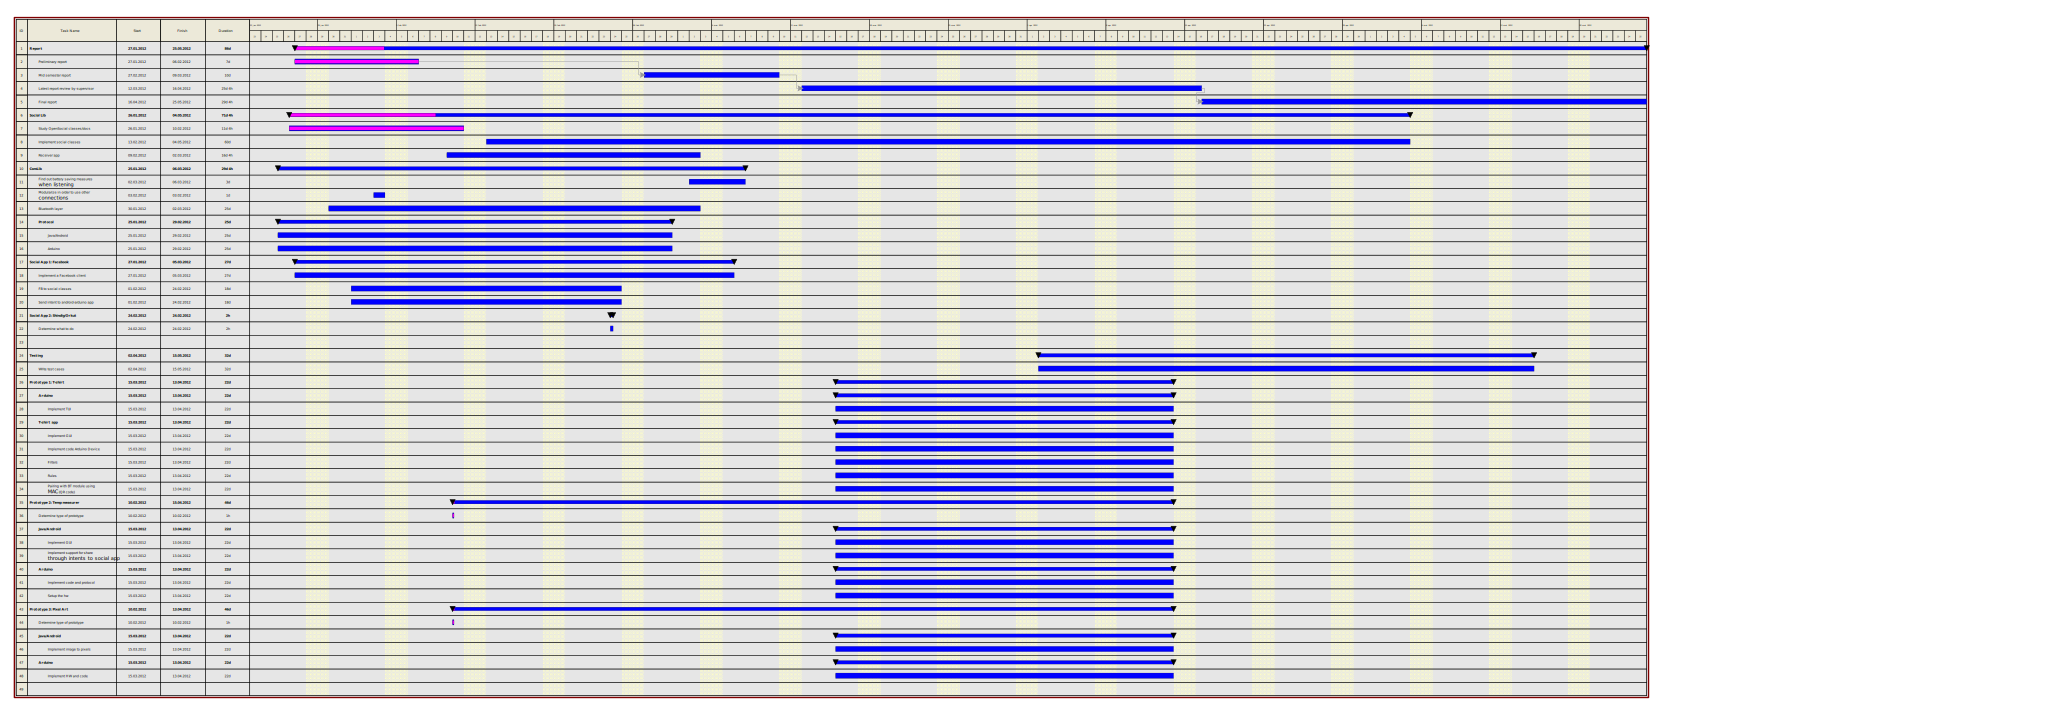
\includegraphics[angle=270, width=1\textwidth, trim=0mm 0mm 47.5cm 0mm, clip]{img/mgmt-gantt.pdf} \caption{Gantt Diagram - part 1}
\label{fig:mgmt-gantt-1}
\end{figure}

\begin{figure}[h]
\centering 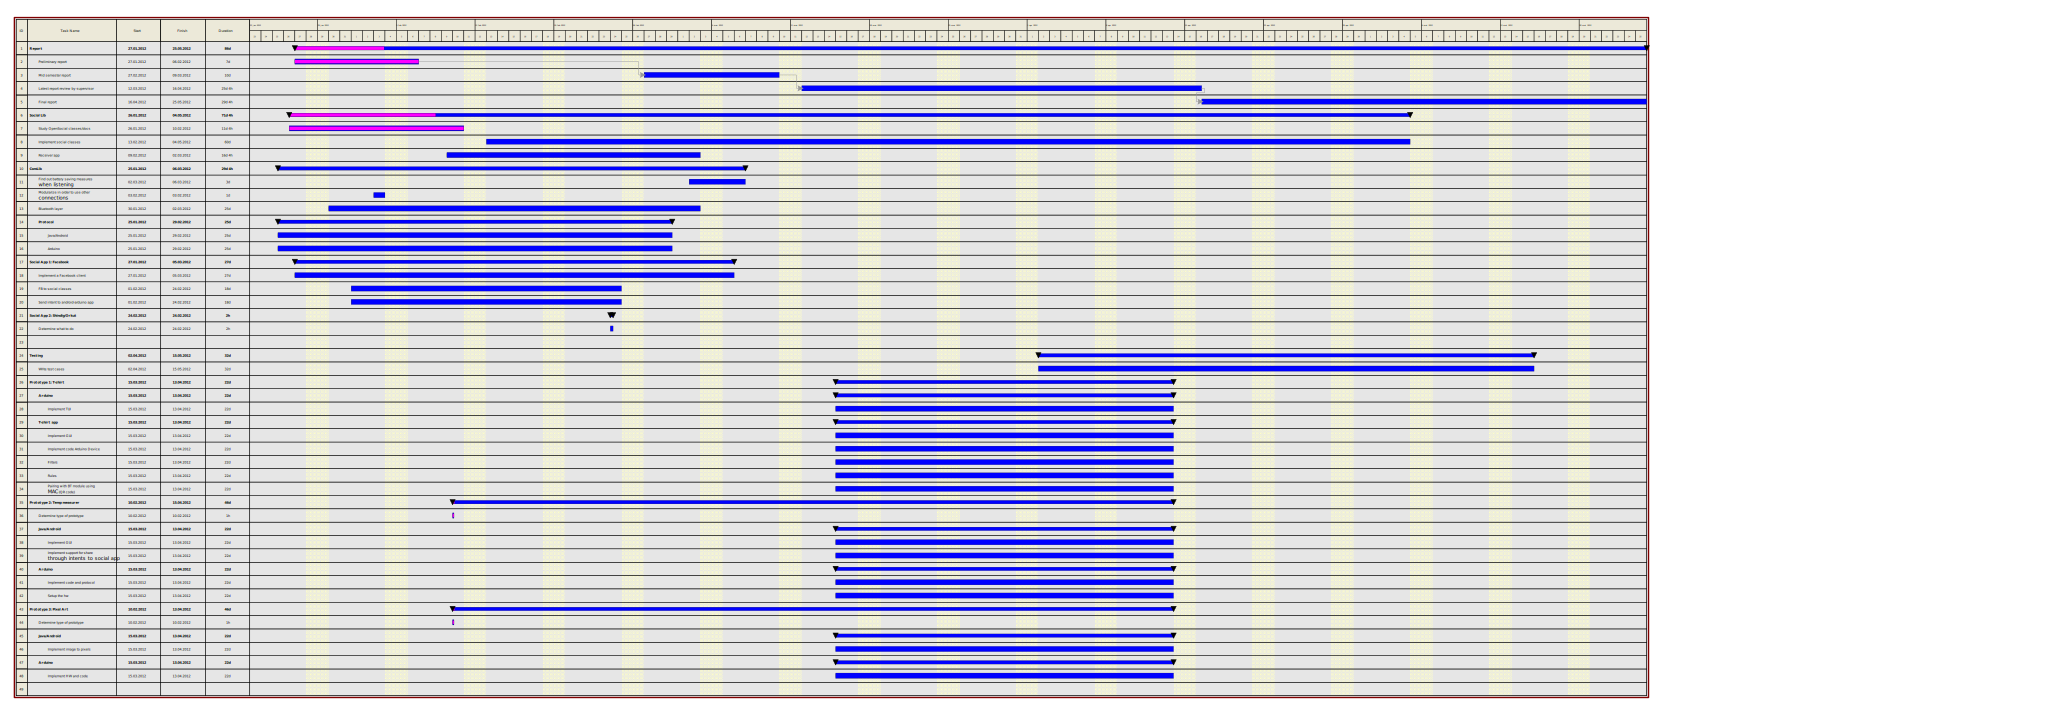
\includegraphics[angle=270, width=1\textwidth, trim=45.5cm 0mm 0mm 0mm, clip]{img/mgmt-gantt.pdf} \caption{Gantt Diagram - part 2}
\label{fig:mgmt-gantt-2}
\end{figure}


\cleardoublepage{}


\chapter{Architecture Design}

\label{ch:architecture} 
\section{First approach}
Our first approach to design the product was to develop:

\begin{itemize}
\item A java 'Social' library that abstracted many common concepts found in different
social networks (Facebook, Twitter, LinkedIn..) like User, Post, Image and so on,
in order to give the developers the possibility to use and extend these concepts seamlessly
between different social networks. It would also handle the connection to the social networks,
to allow the developer to write full-fledged social 'multi-network' clients.

\item A java 'Communication' library to connect, using different interfaces, to the Arduino devices
in order to send the data fetched from the social networks. It would also provide a mechanism to manage
Arduino's firmware, to allow the device to support different hardware configurations.

\item A prototype showcasing the functionalities of the two libraries.
\end{itemize}

After the second meeting with the customer we decided to revise this plan, as this was not what
our customer really had in mind and also a bit ambitious. Some of the code and documentation we produced
earlier could be re-used, but some could not.

See appendix~\ref{app:firstdraftarchi} for more.

\newpage
\section{Revised approach}
The biggest difference in the new approach is that while the Social library will still provide
abstractions for concepts common found in social networks, it will now focus rather than handling
the connection to the social networks, on estabilishing a communication interface (using Android's Intent mechanism)
between Social applications and the Android-Arduino applications to allow them to request and forward 'social' data.

\begin{figure}[h!]
\centering \includegraphics[scale=0.35]{img/architecture-toplevel.png}
\caption{Revised system architecture}
\label{fig:architecture-toplevel}
\end{figure}

\newpage

\subsection{First system design}
Our first system design was based on the scenario where the user would download the t-shirt
and the social applications, browse for some content from within the social application
and actively send it to the t-shirt application pressing a 'share' button.
This scenario is represented in figure \ref{fig:use-case1}

\begin{figure}[h!]
\centering \includegraphics[scale=0.35]{img/architecture-usecase1.png}
\caption{Use case for the first design}
\label{fig:use-case1}
\end{figure}

Different sample applications following this design were developed and showed to the
customer for feedback, and this helped us realize at some point that this design wouldn't fit
the customer ideas for the final product.

\begin{figure}[h!]
\centering \includegraphics[scale=0.35]{img/architecture-resp.png}
\caption{}
\label{fig:resp}
\end{figure}

\subsection{Second system design}
Showing the customer various simple prototype applications in order to receive feedback we would use
to proceed with the system design, we understood that our first design was not really fitting in the
common use-case scenarios that the customer was mentioning.

The user was not supposed to browse for social content and send it actively to the T-Shirt application.
Instead, after downloading the software, he would just setup a set of rules specifying the behavior of the T-Shirt.

This made clear that both the Social and the T-Shirt applications needed to be implemented
as Android services in order to run in background, without user interaction; it also implied 
that a mechanism to specify what content to fetch had to be provided by the Social library.

\begin{figure}[h!]
\centering \includegraphics[scale=0.35]{img/architecture-usecase2.png}
\caption{Use case for the second design}
\label{fig:use-case2}
\end{figure}

\begin{figure}[h!]
\centering \includegraphics[scale=0.35]{img/architecture-reqresp.png}
\caption{?}
\label{fig:reqresp}
\end{figure}

\newpage
\section{Architecture diagram}

\todo{
	needs to be rewritten
}
The API layer is the social service layer. It uses androids build in broadcast intents to send and
recive data to social services. Included in the social service we have classes that extends Intent
class to indicate if its a social Post, social Group, social Image, social User etc. Multiple apps
can use the API layer to send and retrive this data.

Example:
The API layer is connected with twitter. Twitter retrives a new post and the API layer sends out
a broadcast intent marked as $SOCIAL_POST_IN$. The android OS see who are listeneing to $SOCIAL_POST_IN$ and relay the message to all connected apps. The Developed app now has the post. If the developed app wants to send a post it sends an intent with $SOCIAL_POST_OUT$ that our API can pick up.

The bluetooth protocol in the application is a framework that the developed application includes
to be able to send and recive raw data from the arduino board. It includes handshake and
confirmation commands that is similar to tcp.

The arduino board includes a wrapper around the input/output of the firmware to connect to our protocol.

\section{Sequence Diagram}
The sequence diagram shows off a sample run of connecting and requesting information from a social service etc. the t-shirt application requests friendlist from facebook and age of friend 'Anna'.
\newpage
\begin{figure}[h!]
\centering \includegraphics[width=1.0\textwidth]{img/sequenceDiagramSocialService.png} \caption{Sequence Diagram Social Service}
\label{fig:sequenceDiagramSocialService}
\end{figure}

\section{Package Structure}
The system can be divided into smaller sections. This section describes some of the structures
we have divided the system into. The most obvious distinction is between the Java code runs
on the Android platform and the C code which is executed by the Arduino platform.
The Java code is again divided into packaged libraries as described below.

\subsection{Java Code}
\begin{itemize}
\item{no.ntnu.osnap.com}\newline
Communication Library contains every class to establish a connection with a remote device using a general protocol interface. The actual details of the communication such as
Bluetooth, cable, WiFi, stream-based or sockets are hidden away from the user. This is to provide a simple and generic interface to all supported communication methods. The
user can easily add new communication types by extending an abstract class.
\item{no.ntnu.osnap.com.testing}\newline
Test units and sample programs for the ComLib. These are simple test applications that are run on the Android to test if the ComLib is communication correctly using the specified
protocol.
\item{no.ntnu.osnap.social}\newline
Social Library provides an easy to use interface between social networks such as Facebook, Twitter and Myspace and any application or service running on the Android platform.
The SocialLib also provides some general data models such as Person, Group or Post which are concepts that are similar between any social network. 
\item{no.ntnu.osnap.social.testing}  \newline
Test units and sample programs for the SocialLib.
\end{itemize}

\subsection{Arduino C code}
C source code for the Arduino firmware supporting the ComLib protocol.


\cleardoublepage{}


\chapter{Alternative Solutions}

\label{ch:solutions} \section{Existing solutions}

We have done some investigations to other solutions found on the internet. An interesting and very relevant product was a Facebook like indicator that would glow when something you posted was liked. The interesting was that this was done with an Arduino board inside a Lego hand. Another is a mailbox rising it’s arm whenever you got a notification on Facebook. The relevancy for us is that we see it is possible to connect with Facebook in a tangible way using the Arduino. Our own ideas to not have to differ much from already existing concepts, our goal is to show that we can develop a general concept that would encompass these ideas if that was the case. We also looked into other social networks than Facebook like Twitter or LinkedIn. The advantage of other social networks than Facebook is that most use the open source social application API called OpenSocial. Facebook is arguably one of the most popular networks out there, but uses a proprietary API that is not compatible with all the other social networks.

Ultimately we presented various ideas and solutions to the customer and let the customer decide on what they would like to see. As a prototype he would like to see a t-shirt with various signals like LEDS that lighted whenever the user had status updates on Facebook, Twitter or another social network. Major advantage of this solution we can prototype connection to multiple social networks at the same time, so it is a good proof of concept for a tangiable Arduino device connected to multiple social networks.

\cleardoublepage{}


\chapter{Implementation}

\label{ch:implementation} 
\section{Software development tools}

Various software tools will be used througout the project. These include: 
\begin{itemize}
\item Integrated Development Environments: Netbeans and Eclipse 
\item Collabaration tools: git, svn, trac 
\item Pre-existing software: Facebook Android SDK, Android SDK, Twitter4j 
\end{itemize}

\section{Hardware development tools}

The project task requires various hardware, namely Arduino boards,
shields, modules and Android mobiles. Our customer kindly arragend
for us so that we could borrow some Arduino equipment from the lab.
The team used its own mobiles for running, testing and prototyping
the system. 


\cleardoublepage{}


\chapter{System Testing}

\label{ch:systest} 
Testing is an integral part of every development process.
Many different testing approaches have been proposed during the history of
software development, but they all suggest that testing has to be performed continuously
during the development process. This is of particular importance to our process since
it follows an iterative approach. Testing should be planned in the early stages of each
iteration for each testable unit that is going to be implemented and performed as soon as
the iteration is complete. As the system evolves so does the testing. It should be more comprehensive and cover each module and the
system itself as a whole.

\section{Customer feedback}
Customer feedback was an important part of the testing approach for our project.
Working prototypes and/or documentation were produced for each meeting with the customer
in order to test the features implemented in the prototypes, receive a general acceptance
on our iteration goals and plan the next iteration. Receiving a constant feedback from the
user was very important as especially the 'social' part of the project didn't really have a
specific set of requirements from the beginning, so acquiring feedback from the customer allowed
us to understand the most common use case scenarios and from those obtain a set of requirements used
to design the system.

\section{Unit testing}
This involves testing small portions, like methods and functions, of the code, making sure they work 
as intended throughout the process of implementing code. Tests will be executed after changes in the 
code to make sure that it still works as expected, this means that unit tests have to be written for 
large portions of the API.

\section{User interface testing}
For the prototypes we made some applications that will run on an Android phone. To make sure our 
prototypes are understandable and easy to use, we have used group members that have not been 
involved in the process of making the UI, as test candidates. It might not be the ideal way of testing 
an UI, but in the given timeframe of this project it was the easiest and fastest way of doing it.

\section{Integration testing}
After each module of the API has been Unit tested, they will be put together to form bigger components 
of the working system. This is to make sure that the smaller modules will work correctly when placed 
into bigger components. 

In our case this will be to run tests on ComLib and SocialLib making sure they work individually, 
before they are tested together.

\section{System testing}
This involves butting the components from integration testing together to form a complete system that 
can be tested. Preferably each module will be added incrementally, to easier spot if any modules produce errors.

\cleardoublepage{}


\chapter{Results}

\label{ch:results} \input{files/results.tex}

\cleardoublepage{}


\chapter{Discussion}

\label{ch:discussion} \input{files/discussion.tex}

\cleardoublepage{}


\chapter{Conclusion and Further Work}

\label{ch:conclusion} \section{Mistakes and new Experiences}
A big part of projects like this is reflecting back and see which mistakes were made throughout
the project lifetime. We can then learn why these mistakes happened and develop strategies to
prevent them from happening in future projects. This section describes the various pitfalls and
mistakes that were made throughout the project and what we have learned from these.

\subsection{Establishing project requirements}
A lot of time was lost by prematurely starting the design and planning phase before the
requirements were properly understood and established. This was also caused by the shifting 
requirements that the customer had every meeting. We should have properly established a list of
requirements and agreed with the customer that these were the final requirements. In addition we
should have not started major planning, like setting up resource management before the requirements
were properly set after a few meetings with the customer.

\subsection{Hardware problems}
There were various issues with the hardware for our prototypes. A big one was the large delay
from when we initially ordered the hardware and until we received them. It took just over two months for
some of the necessary hardware to arrive, resulting in a delay in our integration and testing process.
This was a major setback to our plans and this time was mostly spent writing documentation, planning
and testing the libraries for bugs. Due to miscommunication within the project group some of the 
hardware we received was either wrong or not quite optimal for our specifications. In addition we had 
not ordered backup or spare parts, so when for example the LCD screen broke, we had to find other 
workarounds to solve this issue. In hindsight we should have made sure that the list of hardware orders 
were correct and ordered additional spare parts in case something broke or malfunctioned.

\subsection{Group meetings}
A chronic problem inside the group was late attendance to internal team meetings. For various reasons members of
the group would meet hours later than the agreed or planned time. This was somewhat mitigated by having 
the meetings later in the day and working into the late hours of the night.

\subsection{Limiting project scope}
A problem caused by an early design choice was the level of portability. Initially we coded our libraries to support as a wide range of platforms as possible (PC, Android, iOS, etc.). This caused various generalizations and concepts that didn't work to well with the Android platform. One prevalent example was callbacks and threads inside the Android system. While our library was based on multi-threading and callbacks through an observer pattern, this does not work on Android Java the same way one would expect on a PC. Since every prototype and testing software we coded was based on the Android platform this caused major problems and we had to spend a lot of time rewriting and redesigning libraries. So our choice of portability caused many problems considering the customer explicitly stated that we only needed to support Android. While portability is usually a good thing, the product quality should not suffer if it is not a high priority requirement.

\section{Further Work}
This section describes ideas, code and features we did not have time or resources to
finish at the project deadline. The section can also describe various interesting concepts 
that we visualized, which we could have explored given more time.

\subsection{Supporting more communication technologies in ComLib}
Currently the ComLib only supports Bluetooth connections. Further work would be
to add support for additional communication technologies such as WiFi and Near Field 
Communication (NFC). The ComLib has been implemented so that this work should
be as easy as possible. Simply extend the Protocol class and implement the input and
output communication and the implementation should be fully forward and backwards
compatible with other versions of the ComLib.

\subsection{Supporting additional Social networks}
The SocialLib currently supports Twitter and Facebook. Support for additional social
networks like Google Plus, LinkedIn or MySpace was planned as future work. The
SocialLib has also been implemented to accommodate this process as simple as possible
for the developer.

\subsection{Multi-Platform}
The Bluetooth part of the ComLib has been implemented using Android SDK. This means that 
the Bluetooth part of the library will only run on an Android platform. The ComLib protocol
itself however, has been designed to support any type of platform. This means the ComLib
could be expanded to support other types of platform such as Bluetooth on iOS. This
should preferably be implemented as a common interface, so that the developer only has to use
Bluetooth, and the ComLib itself figures out if it is to use the Android version or the iOS version of
the Bluetooth Protocol.

\subsection{Security}
Currently the ComLib offers no level of security. Anyone with the mac address can connect
and have access to the full functionality of each prototype device. A future possibility could
be to define a security standard in the ComLib protocol like authentication with a password.

\subsection{ComLib's size parameter}
The ComLib was altered the last week before a presentation to support larger packages. This was to properly
be able to retrieve all metadata from the Arduino. A suggested solution was to ask for the metadata
in several packages, and then merge those packages to get all the metadata. We did not revert the changes
as this was not prioritized in the small amount of time we had left in the project.

\section{Conclusion}
The final scope of the project was much bigger than we originally planned and envisioned. This large scope
was mainly caused because of all the different prototypes we had to implement. Originally we had planned
to implement one prototype with accompanying application, but ended up creating two developer libraries
along with 3 prototypes and 6 different Android applications in addition to a webpage for distribution of oSNAP
compatible software. While challenging this was also a lot of fun, since we had a lot of freedom in developing
these products in the way we liked.

The weekly meetings with the customer proved to be very valuable and
a good way for the customer to keep track of progress. We showed the fruits of our work from the earlier
week to the customer, and he could steer us in the direction he desired and comment on the results.


% ---------------------------------------------------------------------------- %
% Report appendixes goes here


\appendix
%dummy comment inserted by tex2lyx to ensure that this paragraph is not empty
%dummy comment inserted by tex2lyx to ensure that this paragraph is not empty
\appendixpage \addappheadtotoc

\cleardoublepage{}


\chapter{Status Reports}

\label{app:statusreports} \section{Week 4}

First weeks status report where major directional decisions will be explained.

\subsection{Progress summary}
The starting weeks work was mainly focused on identifying the specifics of our task and for every group member to start individual research into possibilities in Arduino, Facebook APIs, other social network APIs and then reporting it back to the group at our meetings. Together we tried to find good concepts for the Tangible User Interface(TUI) product that we was going to make. We had a meeting with the customer on the friday where we discussed our concepts. In this meeting the customer voiced wishes for the project to go in a more general direction than focusing on specific tangible end products. We was going to make a framework where creating products with an Arduino chip was lessened in complexity both for the developer and the end user.
We also got Arduino products(Bluetooth module etc) from Simone Mora from IDI.

\subsection{Open / closed problems}
The direction the project should pursue in regards to the TUI and platform choice became clear on  the meeting with the customer.
How well the Arduino chip could handle wireless connections(Bluetooth, WiFi or Zigby) is an open problem.

\subsection{ Planned work for next period}
In the meeting with the customer we decided on a task for the next period. If we could show that the Arduino could be linked with an Android and/or PC through a wireless connection we could further refine the requirements and goals of the project. 

\subsection{Updated risks analysis}
Wireless connectivity; if the Arduino chip addon modules(called SHIELDS) for Bluetooth etc. was too hard to implement we would have to reconsider wireless connectivity. We set the get "wireless to work" deadline to be one month. Otherwise we would have to use only cabled connections and that would be clumsy on a lot of cool concepts.
 Likelihood: 4 Impact: 6 Importance: 24

\section{Week 5}

A report of a very productive week with some breakthroughs and setbacks.

\subsection{Progress summary}
We started by working on the tasks set forth. We got the Bluetooth module(SHIELD) to work much faster than we had planned for. Therefore we set the bar higher and started working on a general protocol to be used for communication between Arduino and computers regardless of technology (USB,BT,WiFi etc). We also had people working on getting a working Facebook application fetch data from Facebook (last post on Facebook wall). Getting a bluetooth connection between Android and Arduino was also a challenging task that we got working by the end of the week. Our results this week was presented to the customer on the friday as we had agreed on. Our progress relative to our plan is very good, we are actually ahead of schedule.
We also started working on the preliminary report that is due in WEEK 6. We chose to write this in LaTeX language as this is the most powerful way to customise the style of our report. 

In the meeting with the customer we had to revise our plan regarding to the Android framework. The way social networks/applications connect to our framework should be with intents(an Android standard) and that the framework should be highly flexible in regards to which applications it can work on. This lead us to reject some of the code we had made for Facebook fetching, Android Bluetooth talking amongst other things.


We also established working process management tools in GitHub and ScrumDo (www.scrumdo.com). 


\subsection{Open / closed problems}
Closed: wireless connectivity to Arduino is a reality and Bluetooth was decided upon as this is a standard in all mobile smart phones these days so the possibilties are bigger.

Open:
The concept of intents on Android needs to be understood and tried in action.


\subsection{Planned work for next period}
Revise established plans on all levels of our project.
Set the plans in motion.

\subsection{Updated risks analysis}
The risk of wireless connectivity not working is void after this weeks progress.

\section{Week 6}

\input{./files/appendix/weekreports/STATUSREPORTWEEk6.pdf}

\section{Week 7}

\subsection{Progress summary}
This week we had discussions on which development process we should use. Xtreme Programming, spiral and others were considered but we concluded that a modified version of scrum like we previously decided on was feasible. This would also be the most reasonable choice to promote continuity with past work. Other than this we had a slow week with not much progress in regards to programming, rather we focused on process and planning work.

\subsection{Open / closed problems}
Closed: Final decision on using scrum as development/process system. 

Open:
Protocol, bluetooth, social media all need refinement to fit in the scope of the project as it stands.


\subsection{Planned work for next period}
Continue work on all established work packages.

\subsection{Updated risks analysis}
N/A

\section{Week 8}

\subsection{Progress summary}
Further refinement of the communication library. We had some initial planning of several prototypes that would supplement the main T-Shirt idea (T-shirt was replaced by a jacket later in the project). One of them was a LED light Mood indicator fetched from Myspace. We also had more planning and research programming going into the social library, but much work remains to be done on this part.

Open:
ComLib(Bluetooth Arduino-Android comm)
Social Library
Prototypes

\subsection{Planned work for next period}
Finish communication libraries
Decide on design for social library

\subsection{Updated risks analysis}
Redesigning the social library plans too much will limit progress. HIGH risk.


\section{Week 9}

\subsection{Progress summary}
This week much planning and design discussions was had on the social library. Progress was done 
and now the work of implementing some of this is to be undertaken. The communication library 
between arduino and android bluetooth is finished pending further development. The mid-term report is 
due next week, so we started working on that as well.

Open:
Social Library
Prototypes

Closed:
Social library(Facebook, OpenSocial, etc)


\subsection{Planned work for next period}
Finish the mid-term report


\subsection{Updated risks analysis}
There is still a major risk involving the difficulty of finding viable solutions on the social library part of the architecture.


\cleardoublepage{}


\chapter{First draft of the architecture}

\label{app:firstdraftarchi} The client asks for a Java framework that works on either Android or desktop, to support the connection between a Arduino board and social services.

If a programmer wants to use the framework to connect a social service to the Arduino board, he would like to work with data in either end and forward it.

\begin{itemize}
  \item\textbf{Example 1:} 

  He would like to retrieve data from the social service, do something with it, and push data to the Arduino.

  \item\textbf{Example 2:}

  He would like to grab data from the Arduino, do something with it, and upload it to a social service.
\end{itemize}

This illustrates a split in the middle where the developer wants to treat the data himself. Since there is no direct connection between a social service and the Arduino board from our framework, it makes sense to split the framework into two parts.

\begin{itemize}
  \item\textbf{Framework part one:} Retrieving and uploading data between social service and Java.
  \item\textbf{Framework part two:} Grab and push data between the Arduino board and Java.
\end{itemize}

Both frameworks would need to support Android and development. This is an advantage for us who is going to create the framework, and for those who are going to use it.

The disadvantage is that it will be no direct connection from the Arduino board to a social service.
I.e, the board can not connect directly through the Internet to Facebook. It needs a middleman, either a Android phone or a laptop.

After some tests, we have figured out that it makes no difference if the Arduino board is connected through a Bluetooth device or trough an USB cable. If it's an USB cable, the board shows up as a COM port. If the board is paired with the computer/mobile using the operating system/Android, it also shows up as a COM port. So the program searches the COM ports and connects to the board anyhow. (It's may not work on all bluetooth chipsets)


The board needs a firmware that is precompiled on a computer.
That process should be easy for the developer.

\begin{figure}
  \centering
  \includegraphics{./img/architecture-mockupgui.png}
  \caption{An early mockup of the GUI}
  \label{fig:architecture-mockupgui}
\end{figure}

On Create Firmware it should be compiled a file that the developer implements in his Arduino program.

\section{Example run framework part 1}

How the developer connects to board on Android/PC after pairing the Arduino with system.

\javacode
\begin{lstlisting}
//We search the COM ports trying to find the board
Arduinoboard board = Arduinoboard.findBoard();

//We retrive the current firmware name onboardString currentFirmware = board.getFirmwareName();

if(currentFirmware.equals("MyArduinoFirmware"){
    //Everything is OK, the firmware we want is on board.
}
else{
    //There is wrong Firmware/no firmware
    //We upload the one we precreated on our computer.
    File file = new File("/firmwareLocation/firm.fw");
    ArduinoFirmware fw = ArduinoFirmware.getFW(file);

    board.uploadFirmware(fw);
}

//We can see what shields we have according to the premade firmware
ArduinoShield shields = board.getShields();

//Or we can ask for the shield directly
LEDKeyPadShield display = board.getShield(LEDKeyPadShield.class);

//Now the developer can do what he wants with the shields.
display.printText("HelloWorld");
\end{lstlisting}

\clearpage

\begin{figure}[hp]
  \includegraphics{./img/architecture-arduinojava.png}
  \caption{A first sketch of Arduino-Java connection}
  \label{fig:architecture-arduinojava}
\end{figure}

\section{Adding a listener to shield}


Developer adds his listener.
\javacode
\begin{lstlisting}
LEDKeyPadShield display = board.getShield(LEDKeyPadShield.class);
display.addStateChangeListener(new ArduinoStateChangeListener(){
  @Override
   public void stateChanged(ArduinoStateChangeEvent event) {
    if(event.getFlag == LEDKeyPadShield.DOWN){
        //Get down and boogie
    }
   }
});
\end{lstlisting}

In ArduinoConnection we have listenForData(); method, that has its own thread listening on it.

Steps:
listenForData() recives a ArduinoPacked data from Arduino board.

Thread looks in board.shields to find the same board as packet.getName().

It dumps the package into the shield.newArrivalPackage(dataPackage);

It is then up to the shield class to extract the data from package, and fire off an ArduinoEvent to the listeners.


\section{Constant data stream solutions}

Some shields, like the accelerometer is sensitive and will always send data to the program. On a mobile phone who constantly needs to work on these packages this will be straining on the battery.

The constantStream threshold value is a signal to the ArduinoBoard to indicate how often in will update.

Threshold = 0.0f; means all data will be streamed
Threshold = 1.0f; means no data will be send from shield to the program. You can only retrieve data by specifically asking for it.

A mid value is dependent on the Shields connected, if the accelerometer has upper values in x,y,z directions from $<-1000, 1000>$, a threshold of $0.8f$ indicates we need extreme sudden change of $\Delta(0.8*2000)$ in one of the x,y,z axis to send a notification from the Arduino board.

Example, extremely sudden change (In one cycle?) from -700 to +800 in x direction.  

It's not yet clear if we can implement this function into the firmware.

\section{Example run framework part 2}

\javacode
\begin{lstlisting}
//In this case, we register our service with a premade simple Facebook app we have created on
//Facebook.com
SocialService service = new FacebookService(FacebookSevice.getAppAuth("appName"));

//The initateLogin will call up a browser window and request user to log in
//(automatically handle the calls depending if its called from Android or PC)
service.initateLogin();

//Adding listener
service.addSocialListener(new SocialListener(){
  @Override
   public void newPost(Post post) {
    String message = post.message[0];
   }
});

//New post
service.postNewPost(new Post("Hello Profile"));
\end{lstlisting}

\cleardoublepage{}


\chapter{Test}

\label{app:tests} \input{files/appendix/testappendix.tex}

\cleardoublepage{}


\chapter{Meeting minutes}

\label{app:meetings} \section{20.01.2012}

\subsection{Participants}
 Everyone

\subsection{Agenda}
First meeting, Contact the client

Contacted the client: First meeting at Friday 27/01 at 14:00

Send mail to the client with phone numbers/names

Checking free slots in schedule when we can have meetings:

\begin{verbatim}
Monday 12:15 and out
Entire Wednesday
Friday 14:15 and out
\end{verbatim}

\subsection{To do to next meeting}

Everyone:
\begin{itemize}
\item Check solutions for connecting Facebook and Arduino
\item Facebook -- openSocial (Java) -- C/Arduino IDE -- Chipset
\item BrainStorm
\item Make some notes/schemes.
\end{itemize}

Henrik:
\begin{itemize}
\item Read on OpenSocial
\end{itemize}

Jonas:
\begin{itemize}
\item Setup GIT, Mailing list, examine OpenSocial and Shindig
\end{itemize}

Emanuele:
\begin{itemize}
\item Find available Facebook APIs, documents on Open Social, Apache Shindig..
\end{itemize}

Asbjorn:
\begin{itemize}
\item Read on Arduino
\end{itemize}

Anders and Bjørnar:
\begin{itemize}
\item Connect Arduino to Java
\end{itemize}


Johan:
\begin{itemize}
\item OpenSocial, Java $\rightarrow$ Arduino
\item Send two mails:
\item To SINTEF
\item To reception to book room Friday 4th floor at 14:15 every week
\end{itemize}

\subsection{Next meeting}
Monday 23/01 GreenHouse

Discuss brainstorm/possibilities

Get a meeting room at Friday at 14, to meet with the client

\section{23.01.2012}

\subsection{Participants}
Everyone

\subsection{Agenda}
We will probably use the Java Facebook API library restFB. 
Shared some ideas. Discussed a little bit on the development process to use.
Will probably adopt Scrum as development process, given the iterative nature of our work schedule and of the meetings with customer.
Realized a proof of concept consisting of a LED turned on by the Arduino, if there is any unread notifications on Facebook.

{\bf Henrik: } \newline
\begin{itemize}
\item Read on OpenSocial
\end{itemize}

Results
\begin{itemize}
\item Disregard Open Social
\item Idea: Facebook game: Torture instrument at NTNU
\end{itemize}

{\bf Jonas:} \newline
\begin{itemize}
\item Setup GIT, Mailing list, examine OpenSocial and Shindig
\end{itemize}

Results
\begin{itemize}
\item Git and mailing-list up
\end{itemize}

{\bf Emanuele: } \newline
\begin{itemize}
\item Read on available Facebook and other social networks Java API.
\end{itemize}

Results
\begin{itemize}
\item Read the Facebook developers pages (Facebook Graph API, access tokens..)
and Open Social documentation. 
\item It turned out Facebook does not implement the Open Social standard. restFB, a simple, flexible, actively developed and permissively licensed (MIT) Java Facebook API was found and used to code a small program that checks for unread notifications.
\end{itemize}

{\bf Asbjørn: } \newline
\begin{itemize}
\item Read on Arduino
\end{itemize}

Results
\begin{itemize}
\item Idea: Handshake friend request
\item Idea: Camera takes profile picture.
\end{itemize}


{\bf Anders and Bjørnar: } \newline
\begin{itemize}
\item Connect Arduino to Java
\end{itemize}

Results
\begin{itemize}
\item Success!
\end{itemize}

{\bf Johan: } \newline
\begin{itemize}
\item OpenSocial, Java -> Arduino
\item Send two mail
\item To SINTEF
\item To reception to book room Friday 4th floor at 14:15 every week
\end{itemize}

Results
\begin{itemize}
\item Acquired room: 236 it-syd. Every Friday from 14:00 to 17:00
\item Mail sent to client to meet at room next Friday.
\end{itemize}

\subsection{Next meeting}

{\bf Henrik: } \newline
Create idea presentations.

{\bf Jonas and Johan: } \newline
Collaboration tools

{\bf Emanuele: } \newline
Try to find an alternative to polling Facebook. (A callback mechanism?)

{\bf Asbjørn: } \newline
Documentation research

{\bf Anders and Bjørnar: } \newline
Program library for serial Arduino to Java communication

\subsection{Next meeting}
Wednesday 25/01 GreenHouse

Prepare presentations

Implement collaboration tools


\section{03.02.2012}

\subsection{Participants:}
 Everyone present

Meeting started at 14.15


\subsection{Agenda}
Meeting with the customer to show the working prototype according to the specs he had given us.
Talk about issues we had encountered and how they can be fixed.
Presentation of the framework by Henrik.
Get feedback from the customer about what we have done this far, and what he wants us to do next.


\subsection{Additional Information}
Meetings are now moved to 14.15 every Friday, instead of 14.00.
During this meeting the customer had a clearer plan about what the end product should be, and how to get there. This will lead to a rework of the design/plan for this project, but we have a smaller and more specific task to be carried out. This includes making an app/service for the Android OS that uses intents[1] to communicate with other apps on the Android OS.
The use of a custom bootloader for the Arduino is postponed until further notice.


\subsection{ To do for next meeting}
Everyone have to read up on Android Intents and get a basic grasp of the functionality of the Open Social API.
Finish the preliminary report that is due for Monday.
Read up on NFC, find a way we can use it to for example establish connection between a phone and an Arduino device.


\subsection{ To do for next meeting with the customer}
Find out how to separate and use the intents
Make an API to communicate with Android apps through intents, and send this information using bluetooth to an Arduino device.
The API should be able to support different modules(t-shirt, mailbox, etc)
If we have time for it, simulate the use of QR codes to download an app to the phone.
Write a list of what we have to order to make the product/prototype.

Intents can be used to signal to the Android system that a certain event has occurred. Other components in Android can register to this event and will get notified.

\section{10.02.2012}

\subsection{Participants:}
Everyone present everyone except Asbjørn who had notified he would be gone.

Meeting started at 14.15

\subsection{Agenda}
Present how we have understood the task to the customer and get feedback on that.
Get more information about what Mr. Babak wants us to do, and how it should be done.

\subsection{Additional Information}
Mr. Farshchian wants us to make a couple of simple prototypes, then a big one that will show that our API support more than one social media. This will include using two different social apps the Android phone, for example Facebook and Shindig.

He also wants the API to support communication from the Arduino to Android, for example temp reading or you can push a button and poke a predefined person.

We dont have to use the Open Social java classes, but we should look into the concepts of it and do something similar.

Open Social concepts:
\begin{enumerate}
\item  User
\item Group
\item  Post
\item Stream; user stream and group stream.
\item Group activity streams
\end{enumerate}

Would be nice if the communication library could support other ways of communication than just Bluetooth. There should also be a way to pair the Android app with the Arduino by using MAC address.


Gui/Settings in the t-shirt app.


\subsection{To do for next meeting}
Think about how the WBS can be translated to stories, then to tasks for each sprint.

\subsection{To do for next meeting with the customer}
To do Monday:
Talk with Simone about the shopping list, find out what is already available for us.
Check out battery drain

\subsection{Notes from Henrik:}
Two simple prototype and one more advanced prototype

Intents library
Class intents
Stream(timeline)
Group
                
GroupStream
Post
User                

Request Intents
Callbacks
Documentation for intents in Android style

Communication Library
C Wrapper
Find and connect module

Two Social apps

Look at battery drain

near field communication?

Marked integration into last years group project

\subsection{Notes from Bjørnar}
Meeting started @ 14.15

Everyone except Asbjorn present. (notified he would be away)

Talk to the customer that we have had some problems understanding what he wants us to do, and that we want to  make sure that we have understood him correctly before we go from this meeting.

Johan and Emanuel explaining on the whiteboard:
\begin{itemize}
\item Social apps, communicate with intents with our API then to the android/arduino app, the android/arduino app will communicate with bluetooth through our com-layer.
\item What objects that we want to use, defined from the open social standard
\item Up for discussion: how strictly we should follow the open social standard
\item Follow the overall concepts that open social is using
\item API layer will provide parsing from intents to intents.
\item The API is a part of the android/arduino app
\item Use the intent services that are already there, try to specialize the intents for our use
\item Someone who made an app store last year, check into it, can upload any files to it. Student project.
\item UBI home app
\end{itemize}

Henrik is asking about how to make requests from for example t-shirt to the social app:
\begin{itemize}
\item In the library you will have specific things you can ask about, the t-shirt can send intents, but if it wants to use our intents, have for example osnap.* infront of it
\item Look up how to register the app for showing up in menu when you want to share anything
\item Talk with Simone about the shopping list
\end{itemize}

Johan explaining about the extended the t-shirt prototype:
\begin{itemize}
\item QR, bluetooth, supporting more than one social network
\item Extra hw devices that we have thought about, vibration, sound, display, leds
\item News feed to sound, settings page for the t-shirt app, for what should be doing what on the t-shirt
\item Disable/enable modules, what goes where.
\end{itemize}

How to go the other way? \newline
Temp sensor for example, post temp to facebook.
  
Think about if you can make the t-shirt app in a visual editor \newline
To custom make your own t-shirt, related to next phase, not priority (qued)

Have to think about, make a list of specifics of what we want to do. \newline
The t-shirt app, would be cool with more than one thing. Make a couple of simple prototypes, and one big one.
Point is to show that we can do more than one thing, proof it's not hard coded.

Anders talking about the bluetooth:
\begin{itemize}
\item How to connect to a specific bt device
\item Every bt have a mac adress, can be send with the QR code.
\end{itemize}

Communication library:
\begin{itemize}
\item Documentation of the intents, how they work etc.
\item Currently have two simple apps, one sending and one recieving.
\item Social intents library, t-shirt app, talk with group 11 about fall detection??
\item Two social apps, social library, communication library, android apps for prototypes, and firmware for the arduino, documentation for the android action intents, make available on the open source market.
\item Communication library, should it be just BT, or do we have to support other wireless communications?
\item Currently it is transparent, should be possible to implement other kinds of wireless comms later.
\item Wifi would be nice, for example hotspot, so the t-shirt can be internet available.
\item Think about it, not critical
\item NFC tags at the lab, so it would be possible to test it out.
\end{itemize}

Misc:
\begin{itemize}
\item Important to be under Apache license. End user contribution agreement.
\item Look into the market, we will have to get client, and how it works with QR codes etc.
\item Shindig, folder with open social concepts implemented as java classes
\item Some kind of management tool, to remove/update etc
\item Customer want the meeting report agenda.
\end{itemize}


\section{13.02.2012}

Participants: Anders, Bjoernar, Henrik and Johan

Meeting started at 14.15

Agenda
Get feedback on the preliminary report.

Additional Information
Meetings with the student assistant will be held every two weeks, if we are not at P15, we have to remember to notify him. 


Team member roles have to be assigned, each member should also write something about themselves (background, experience/knowledge, what work you have done earlier and stuff like that)


Add more information about why we have chosen Scrum, write something about other development models (Waterfall, Spiral, Agile, Iterative etc) and why we didnt choose to use them. Should also include more about how we have adapted Scrum to our needs.


The status reports should be renamed to the sprints?

Alternate/existing solutions can be put under the pre-studies chapter.


The report should be restructured a bit. See the mail for additional info.


1. Introduction
1.1 The context
1.2 The Customer

2. Process Management
2.1 Process methodologies
2.2 Our choice
2.3 The team
2.4 Project management tools
2.5 Risk analysis and migration strategies
2.6 Schedule (Gant Diagrams, WBS etc)


3. Pre-study
3.1 Communication resources
3.2 Time resources
3.3 Existing solutions
3.4 Software and hardware development tools
3.5 Add more pre-study

4. Requirements
4.1 Functional requirements
4.2 Non functional requirements

5. Architecture Design
5.1 First approach
5.2 Revised approach
5.3 Architecture diagram
5.4 Use cases

System testing, results etc..

\section{17.02.2012}

Participants: Everyone present

Meeting started at 14.20

Agenda
General meeting with Mr. Farshchian, not much programming done or something to show. Talk about what we have done the last week planning wise.

Additional Information
We can check out openintents.org to see if there are something similar out there that we can use for our project.
Stop using opensocial classes and construct our own for the social side.

To do for next meeting

To do for next meeting with the customer
Get the Apache license forms, and sign them.

\section{24.02.2012}

\subsection{Participants}
Everyone present

Meeting started at 14.15

\subsection{Agenda}
Show the GUI for the t-shirt app.
Show and tell about the progress that have been made.
Discuss the usability of Open Social Classes.

\subsection{Additional Information}
If possible our API should be backwards comtabible with the OpenSocial classes, in such a way that developers don’t have to learn a new system when porting from OpenSocial.
Could also look into the activity streams standard?

\subsection{To do for next meeting}
Start working on assigned tasks.
Monday: Fix the shopping list with links to robonor.no

\subsection{To do for next meeting with the customer}
Get the Apache license forms, and sign them.
Start work on connecting all the parts of the project atm, T-shirt app with Social app through Arduino.

\section{29.02.2012}

\subsection{Participants}
Everyone present

Meeting started at 14.15

\subsection{Agenda}
Update studass with our progress and the road ahead.

\subsection{Additional Information}
The studass says we should prioritise the mid-term report and comes with suggestions on what to include in it. 
\begin{itemize}
\item Testing plan
\item Architecture design
\item Requirements must be complete
\end{itemize}


\section{02.03.2012}

Participants: Everyone except Bjoernar present.


Meeting started at 14.15




Agenda
Show the structure of the social API and how it interacts with the various parts on an Android-Arduino system.
Show prototype 3: Wearable pixels.




Additional Information








To do for next meeting
Work on mid-term report


To do for next meeting with the customer
Work on mid-term report will be prioritised, so we can not show progress to the customer in the next meeting.

\cleardoublepage{}  \bibliographystyle{plain}
\bibliography{it2901}

\end{document}
